\begin{tabular}[ht]{M{2cm}M{8cm}M{1cm}M{1cm}}
  %\setlength\extrarowheight{2.5pt}
  \hline
   Particles & Position of particles in cell $c$ & DCU & CTU \\
  \hline
  \hline
  2 & 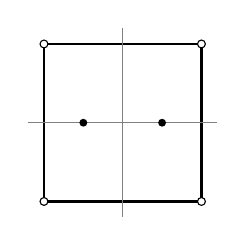
\begin{tikzpicture}[scale=1.]
    \draw[thick] (-1.,-1.) rectangle (1.,1.);
    \draw[black!50] (-1.2,0.) -- (1.2,0.0);\draw[black!50] (.0,-1.2) -- (0.,1.2);
    %% nodes
    \fill[white] (-1,-1) circle (0.05);\draw (-1,-1) circle (0.05);
    \fill[white] (1.,-1) circle (0.05);\draw (1,-1) circle (0.05);
    \fill[white] (1,1) circle (0.05);\draw (1,1) circle (0.05);
    \fill[white] (-1.,1) circle (0.05);\draw (-1,1) circle (0.05);
    %% particles
    \fill[black] (-0.5,0.) circle (0.05);
    \fill[black] (0.5,0.) circle (0.05);
  \end{tikzpicture} 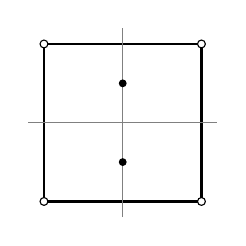
\begin{tikzpicture}[scale=1.]
    \draw[thick] (-1.,-1.) rectangle (1.,1.);
    \draw[black!50] (-1.2,0.) -- (1.2,0.0);\draw[black!50] (.0,-1.2) -- (0.,1.2);
    %% nodes
    \fill[white] (-1,-1) circle (0.05);\draw (-1,-1) circle (0.05);
    \fill[white] (1.,-1) circle (0.05);\draw (1,-1) circle (0.05);
    \fill[white] (1,1) circle (0.05);\draw (1,1) circle (0.05);
    \fill[white] (-1.,1) circle (0.05);\draw (-1,1) circle (0.05);
    %% particles
    \fill[black] (0.,-0.5) circle (0.05);
    \fill[black] (0.,0.5) circle (0.05);
  \end{tikzpicture} &  0.27 & 0.28\\ %%% SOLUTION
  \hline
  2 & 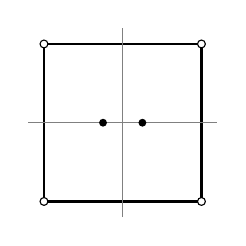
\begin{tikzpicture}[scale=1.]
    \draw[thick] (-1.,-1.) rectangle (1.,1.);
    \draw[black!50] (-1.2,0.) -- (1.2,0.0);\draw[black!50] (.0,-1.2) -- (0.,1.2);
    %% nodes
    \fill[white] (-1,-1) circle (0.05);\draw (-1,-1) circle (0.05);
    \fill[white] (1.,-1) circle (0.05);\draw (1,-1) circle (0.05);
    \fill[white] (1,1) circle (0.05);\draw (1,1) circle (0.05);
    \fill[white] (-1.,1) circle (0.05);\draw (-1,1) circle (0.05);
    %% particles
    \fill[black] (-0.25,0.) circle (0.05);
    \fill[black] (0.25,0.) circle (0.05);
  \end{tikzpicture} 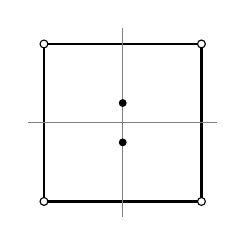
\begin{tikzpicture}[scale=1.]
    \draw[thick] (-1.,-1.) rectangle (1.,1.);
    \draw[black!50] (-1.2,0.) -- (1.2,0.0);\draw[black!50] (.0,-1.2) -- (0.,1.2);
    %% nodes
    \fill[white] (-1,-1) circle (0.05);\draw (-1,-1) circle (0.05);
    \fill[white] (1.,-1) circle (0.05);\draw (1,-1) circle (0.05);
    \fill[white] (1,1) circle (0.05);\draw (1,1) circle (0.05);
    \fill[white] (-1.,1) circle (0.05);\draw (-1,1) circle (0.05);
    %% particles
    \fill[black] (0.,-0.25) circle (0.05);
    \fill[black] (0.,0.25) circle (0.05);
  \end{tikzpicture} &  0.43 & 1.00\\
  \hline
  4 & 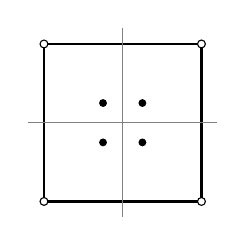
\begin{tikzpicture}[scale=1.]
    \draw[thick] (-1.,-1.) rectangle (1.,1.);
    \draw[black!50] (-1.2,0.) -- (1.2,0.0);\draw[black!50] (.0,-1.2) -- (0.,1.2);
    %% nodes
    \fill[white] (-1,-1) circle (0.05);\draw (-1,-1) circle (0.05);
    \fill[white] (1.,-1) circle (0.05);\draw (1,-1) circle (0.05);
    \fill[white] (1,1) circle (0.05);\draw (1,1) circle (0.05);
    \fill[white] (-1.,1) circle (0.05);\draw (-1,1) circle (0.05);
    %% particles
    \fill[black] (-0.25,-0.25) circle (0.05);
    \fill[black] (0.25,-0.25) circle (0.05);
    \fill[black] (0.25,0.25) circle (0.05);
    \fill[black] (-0.25,0.25) circle (0.05);
  \end{tikzpicture} &  0.43 & 1.00\\%[8pt]
  \hline
  %\begin{minipage}{0.85\textwidth}\lipsum[1]\end{minipage}
\end{tabular}

%%% Local Variables: 
%%% mode: latex
%%% TeX-master: "../../mainManuscript"
%%% End: